\newpage
	\section{Группа движений евклидовой плоскости}
		
		\subsection{ГЛ2 1}		
		Пусть $O_3 = S_{O_2}(O_1)$. Легко проверить, что $S_{O_3} = S_{O_2} \circ S_{O_1} \circ S_{O_2}$. Поэтому если $O_1$ и $O_2$ — центры симметрии фигуры, то и $O_3$ — центр симметрии, причем $O_3 \ne O_1$ и $O_3 \ne O_2$.\\
		
		\subsection{ГЛ2 2}		
		Заметим, что есть 2 последовательности преобразований: отражение $\circ$ поворот и поворот $\circ$ отражение\\
		В (1) случае $s \mapsto s \mapsto s_1$, так как при повороте $s$ переходит в себя, а при отражении $s \mapsto s_1$\\
		Во (2) случае $s \mapsto s_1 \mapsto s_2$, так как при отражении $s \mapsto s_1$, а при повороте $s_1 \mapsto s_2$ (так как приповороте сохраняется только $s$)\\
		Если поворот и отражение коммутируют, то $s_1 = s_2 \: \Rightarrow \: s_1$ лежит на прямой $\Rightarrow \: s$ лежит на прямой, т.е. мы доказали, что если преобразования коммутируют, то $s \in l$\\
		\\
		Теперь докажем обратное - т.е. что если центр симметрии на прямой, то преобразования коммутируют.\\
		Рассмотрим те же 2 случая:\\
		Пусть наша прямая перпендикулярна оси координат x, тогда рассмотрим любую точку на этой оси - по координате x она не сдвинется(так как если рассматривать все по координате x, то оба преобразования просто отражаеют точку, а два отражения $= Id$), а по оси $y$ она сдвинется на $2|y_1 - y_s|$, где $y_1$ координата по $y$ рассматриваемой точки, а $y_s$ координата по $y$ точки $s$), тогда эти композиции движений коммутативны, так как положения точек при обоих последовательностях преобразований совпали.
		
		\subsection{ГЛ2 3}		
		$\text{(в)} \Rightarrow \text{(а)}$ и $\text{(в)} \Rightarrow \text{(б)}$ --- можно просто нарисовать каждый из случаев и разобрать, куда переходят точки при отражениях относительно этих прямых. В случае параллельности оба пункта((а) и (б)) очевидновыполнены. Если же все прямые проходят через одну точку, то $\sigma_{l_1} \circ \sigma_{l_2} \circ \sigma_{l_3} \: = \: \sigma_{l_3} \circ \sigma_{l_2} \circ \sigma_{l_1}$ так как $\sigma_{l_1} \circ \sigma_{l_3} \: = \: \sigma_{l_3} \circ \sigma_{l_1}$ можно рассмотреть как поворот, а $\sigma_{l_2}$ - отражение. Также $\sigma_{l_1} \circ \sigma_{l_2} \circ \sigma_{l_3}$ - симметрия, так как длины сохранились, ориентация изменилась.\\
		$\text{(а)} \Rightarrow \text{(в)}$ 
		
		
		\subsection{ГЛ2 4}		
		A)\\
		Пусть $l$ - отражение относительно прямой, $\overrightarrow{v}$ сдвиг относительно вектора, где $v = v_1 \cdot a + v_2 \cdot b$ - $v_1 \parallel l$ и $v_2 \perp l$. Тогда движение это симметрия со сдвигом $v_1 \cdot a$ относительно прямой $l + \frac{v_2 \cdot b}{2}$. Заметим, что если рассмотреть базис $(0,\: v_1,\:  v_2)$, то движение переводит точку $(x_1,\:  x_2)$ в $(x_1 + a,\:  2l - x_1 + v_2 \cdot b) \: = \: (x_1 + a,\:  2(l + \frac{v_2 \cdot b}{2}) - x_1)$, поэтому оба движения одинаковы.
		\\
		B)\\
		\\
		\subsection{ГЛ2 5}	
		A)\\
		Заметим, что поворот переводит точку $x$ в $(x - a) \cdot e_\alpha + a \: = \: x \cdot e_\alpha + a \cdot (1 - e_\alpha)$, где $a$ - центр поворота, $e_\alpha \: = \: \cos\alpha + i \cdot \sin\alpha$. \\Тогда два повотрота переводят $x$ в $x \cdot e_\alpha \cdot e_\beta + a \cdot (1 - e_\alpha) \cdot e_\beta + b \cdot (1 - e_\beta)$. Тогда если $e_\alpha e_\beta = 1$, то преобразование является сдвигом на вектор $a \cdot (1 - e_\alpha) \cdot e_\beta + b \cdot (1 - e_\beta)$. Если же $e_\alpha e_\beta \: \ne \: 1$, то преобразование это поворот относительно $\frac{a \cdot (1 - e_\alpha) \cdot e_\beta + b \cdot (1 - e_\beta)}{1 - (e_\alpha \cdot e_\beta)}$ на $(e_\alpha \cdot e_\beta)$, то есть на $\alpha + \beta$
		\\ \\
		B)\\
		%\begin{comment}
		Заметим, что симметрия переводит $x$ в $\overline{\frac{x - a}{e_\alpha}} \cdot e_\alpha + a \: = \: \overline{x} \cdot \frac{e_\alpha}{\overline{e_\alpha}} + a \cdot (1 - \frac{e_\alpha}{\overline{e_\alpha}}) \: = \: \overline{x} \cdot e_{2\alpha} + a \cdot (1 - e_{2\alpha})$, где прямая вида $x \: = \: k \cdot e_\alpha + a$ для комплексного $x$ и вещественных $k$ и $a$.\\
		Тогда 2 скользящие симметрии переводят $x$ в $x \cdot \overline{e_{2\alpha}} \cdot e_{2\beta} + \overline{a \cdot (1 - e_{2\alpha})} \cdot e_{2\beta} + b \cdot (1 - e_{2\beta}) + \overline{v_1} \cdot e_{2\beta} + v_2$ что является сдвигом при $\overline{e_{2\alpha}} \cdot e_{2\beta} \: = \: 1$, то есть если прямые параллельны. Сдвиг $\overline{a \cdot (1 - e_{2\alpha})} \cdot e_{2\beta} + b \cdot (1 - e_{2\beta})+ \overline{v_1} \cdot e_{2\beta} + v_2$. При $\overline{e_{2\alpha}} \cdot e_{2\beta} \ne 1$ это поворот на угол $e_{2\alpha} \cdot e_{2\beta}$, то есть $2\alpha + 2\beta$, и центр - $\frac{\overline{a \cdot (1 - e_{2\alpha})} \cdot e_{2\beta} + b \cdot (1 - e_{2\beta})+ \overline{v_1} \cdot e_{2\beta} + v_2}{1 - e_{2\alpha} \cdot e_{2\beta}}$		
		%\end{comment}
		\subsection{ГЛ2 6}		
		A)\\
		Пусть задан треугольник $ABC$, серединные перпендикуляры выбираются в следующем порядке: $AB$, $BC$, $CA$. Тогда точка $A$ переходит после этой композиции в себя, точка пересечения серединных перпендикуляров $O$ также переходит в себя, откуда следует, что для композиции прямая $AO$ - неподвижна, при этом прямые пересекаются в одной точке, значит композиция - отражение, откуда следует, что это отражение относительно прямой $AO$.
		\\ \\
		B)\\
		Пусть треугольник $ABC$, биссектрисы выбираются в следующем порядке: $AI$, $BI$, $CI$, где $I$ - пересечение биссектрис. Тогда проекция $I$ на $AC$ ($B_I$) переходит после этой композиции в себя (определим точки $A_I$ и $C_I$ аналогично, тогда $B_I \mapsto C_I \mapsto A_I \mapsto B_I$), точка пересечения биссектрис $I$ также переходит в себя, откуда следует, что для композиции прямая $B_I I$ - неподвижна, при этом прямые пересекаются в одной точке, значит композиция - отражение, откуда следует, что это отражение относительно прямой $B_I I$.
		\\ \\
		C)\\
		Пусть квадрат $ABCD$. Также пусть порядок отражения следующий: $AB$, $BC$, $CD$, $DA$. Заметим, что композиция отражений относительно $AB$ и $BC$  $\Leftrightarrow$ повороту на $180^\circ$ относительно $B$, аналогично для композиции $CD$ и $DA$ $\Leftrightarrow$ повороту на $180^o$ относительно $D$, откуда следует, что композиция относительно 4 сторон $\Leftrightarrow$ композиции поворотов относительно $B$ и $D$, что равно параллельному сдвигу в сторону удвоенного вектора $\overrightarrow{BD}$.
		
		\subsection{ГЛ2 7}		
		
		
		\subsection{ГЛ2 8}		
		A)\\
		\\
		B)\\
		\\
		C)\\
		\\
		
		\subsection{ГЛ2 9}		
		Пусть треугольник $ABC$ построен: $A$ на $l_{1}$, $B$ на $l_{2}$, $C$ на $l_{3}$. При повороте на $60^{\circ}$ вокруг $A$, тогда $C \to B$, $l_{3} \to l$, тогда точка пересечения $l_2$ и $l$ - $B$.
		Тогда возьмём на $l_{1}$ точку $A$. Образ прямой $l_{3}$ при повороте на $60^{\circ}$ вокруг $A$ пересекает $l_{2}$ в $B$
		\begin{figure}[h]
			\center{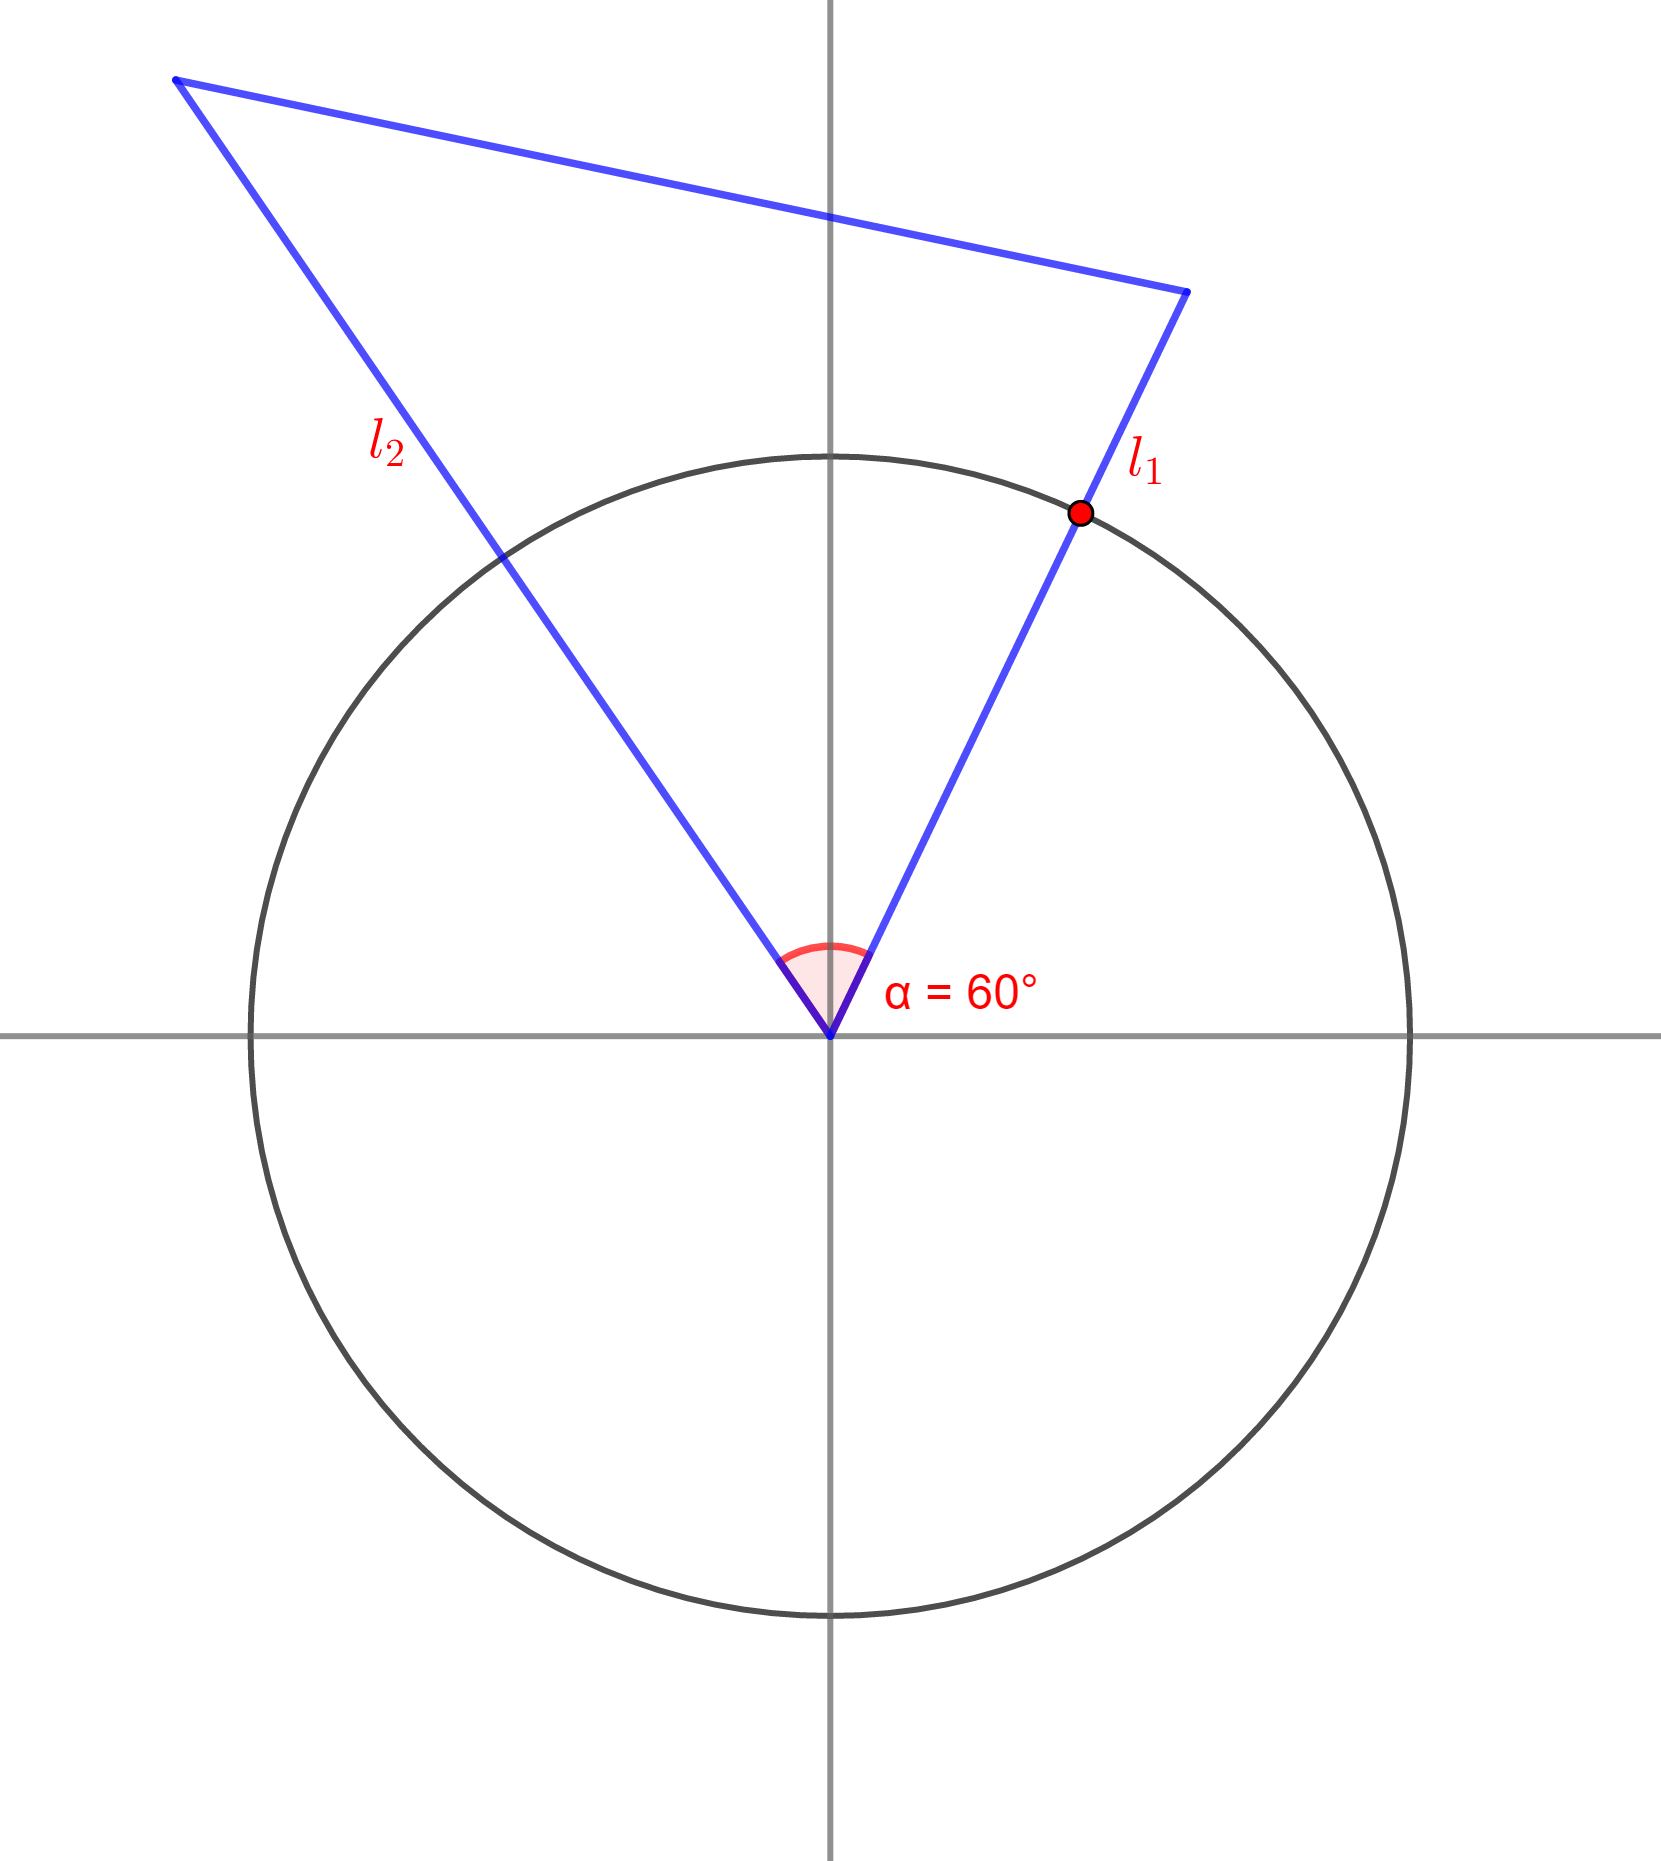
\includegraphics[width = 0.75\linewidth]{Pic2}}
		\end{figure}